\newpage
\section{Problema 2: Algoritmo Exacto para List Coloring}

\subsection{Descripción de la problemática}
En esta oportunidad se nos pide resolver el problema List Coloring que consiste en (si es posible) colorear un grafo de forma que ningún nodo tenga el mismo color que un nodo adyacente, respetando la lista de colores de cada nodo, lo cual quiere decir que no se le puede asignar un color a un nodo si este no pertenecía a su lista de colores posibles. 

\subsection{Resolución propuesta y justificación}

Para desarrollar un algoritmo exacto para este problema decidimos usar backtracking y de esta forma recorrer todas las opciones de colores y poder encontrar la solución si esta existe.\\

Como el enunciado pide que al llegar a un caso de 2-List Coloring se utilice el algoritmo del primer punto, decidimos cambiar el enfoque de la resolución para poder adaptarlo a instancias del ejercicio 1. Por lo tanto en lugar de usar la forma mas convencional de backtracking, que sería fijar un color para cada nodo y ver si es solución, optamos por recorrer todos los nodos del grafo fijando dos colores por cada uno y al llegar al último nodo llamar a 2-list Coloring para que chequee si con esa configuración de colores hay solución. Si la respuesta es $"X"$ entonces se seleccionan los dos colores siguientes del último nodo y se vuelve a probar. Cuando se acaban los colores del último, se elije los próximos colores del ante último y se vuelve a empezar de cero con los colores del siguiente y así hasta que se prueben todos los colores de todos los nodos. De esta forma siempre se llega a un caso base que es resoluble por 2-List Coloring.\\

Para evitar repetir o saltear colores se utiliza un iterador (\emph{it}) que siempre arranca desde el primer color de la lista y dentro del \texttt{while} se seleccionan dos colores consecutivos si hay o se selecciona uno solo (ver pseudocódigo de la sección \ref{sec:complj}) y luego se llama recursivamente a ListColoring para seleccionar los colores del nodo siguiente.\\

A continuación ilustramos la forma en la que se construye el árbol de soluciones para la siguiente lista de nodos:

\begin{center}
\emph{Grafo:} $\{ A, B, C, D \}$\\
Cada nodo tiene la siguiente cantidad de colores: $A: 2$, $B:4$, $C:5$ y $D:6$
\end{center}

\begin{center}
\begin{tikzpicture}[level 1/.style={level distance=1.5cm}]
\Tree
[.{A:0,1}
	[.{B:0,1}
		[.{C:0,1}
			[.{D:0,1} \texttt{2LC} ]
			[.{D:2,3} \texttt{2LC} ]
			[.{D:4,5} \texttt{2LC} ]
		]
		[.{C:2,3} {\vdots} ]
		[.{C:4} {\vdots} ]
	]
	[.{B:2,3}
		[.{C:0,1} {\vdots} ]
		[.{C:2,3} {\vdots} ]
		[.{C:4} {\vdots} ]
	]
]
\end{tikzpicture}
\end{center}

Como se puede observar en la imagen, cada nivel representa los llamados de \emph{ListColoring} para un determinado nodo y se puede ver como se seleccionan los índices de la lista de colores de a dos de forma que en las hojas se llama a \emph{2-List Coloring} (\texttt{2LC}) con todas las combinaciones de colores.

\subsubsection{Podas}

\begin{itemize}
	\item La primer poda que se realiza es la de ordenar la lista de nodos de forma que queden primero los nodos con menor cantidad de colores ya que de esta forma si se eligen los colores de un nodo $a$ con dos colores primero y luego se pasa a uno $b$ de cinco, se estaría recorriendo el subgrafo que no contiene a $a$ dos veces en lugar de las cinco que se recorrería si estuviera primero el nodo $b$.
	
	\item Al revisar el código de la primer entrega nos dimos cuenta que no era necesario hacer todas las permutaciones de los colores de un nodo ya que alcanzaba con seleccionar una sola vez cada color para cada nodo y llamar a 2-List Coloring dado que la recursión se encarga de que los colores se prueben todos con todos.
	
	\item Si se llega a una solución, se corta el backtracking y se devuelve esa. De esta forma en el caso promedio y mejor, no se recorrería todo el árbol de soluciones ya que no necesita encontrar todas las posibles.
\end{itemize}

Por lo tanto como se está generando el árbol de soluciones completo y las podas cortan ramas solo cuando se encontró un coloreo posible o cuando se determina que no existe coloreo, se puede decir que nuestro algoritmo es correcto.

\subsection{Análisis de la complejidad}
\label{sec:complj}

Para analizar la complejidad utilizaremos el siguiente pseudocódigo, en el cual se utilizan los términos definidos a continuación:
\begin{itemize}
	\item \texttt{grafo}: para referirse al que viene por parámetro.
	
	\item \texttt{grafo2colores}: para el grafo que se construye para pasarselo al algoritmo del problema 1 y que admite hasta 2 colores por nodo.
	
	\item \texttt{ListColoring}: es el algoritmo que estamos analizando y representa el llamado recursivo a la misma función. 
	
	\item \texttt{2ListColoring}: es el algoritmo del problema 1 y se usa para obtener la solución a un grafo con a lo sumo dos colores por nodo.
	
	\item $count$: es una variable pasada por parámetro que se utiliza para avanzar y retroceder en la lista de nodos.
	
	\item $c$: es la cantidad máxima de colores que puede tener un nodo y que está dada por la entrada del problema.
\end{itemize}

Como queremos analizar el peor caso, mostraremos las complejidades para el algoritmo sin podas, ya que de esta manera nos aseguramos de que siempre se recorra todo el árbol de soluciones del backtracking.
\newline

\begin{algorithm}[H]
\caption{ListColoring Exacto Sin Podas}
\label{lce}
\begin{algorithmic}[1] 

\STATE $count = $ índice en la lista de nodos del \texttt{grafo} (inicializada en cero, viene por parámetro)

\IF {$count ==$ cantidad de nodos del \texttt{grafo}}
	\STATE Llamar a \texttt{2ListColoring} para resolver \texttt{grafo2colores} \COMMENT{$\mathcal{O}(n^2 \log{n})$} %complejidad del 1
	\STATE Retornar 
\ENDIF

\STATE $nodo = $ Obtener el nodo a procesar del \texttt{grafo} con el índice $count$ \COMMENT{$\mathcal{O}(1)$} \label{get1}
\STATE $it = $ Obtener un iterador de la lista de colores de $nodo$ \COMMENT{$\mathcal{O}(1)$} \label{it}
\STATE $coloresSeleccionados = $ Obtener la lista de colores del $nodo$ en el \texttt{grafo2colores} \COMMENT{$\mathcal{O}(1)$} \label{get2}
\STATE Incrementar $count$ \COMMENT{$\mathcal{O}(1)$}

\WHILE[$\mathcal{O}(c/2)$ en cantidad de ejecuciones.]{Haya próximo en la lista de colores} \label{hn}
	\STATE $color1 = $ Próximo en la lista \COMMENT{$\mathcal{O}(1)$} \label{next}
	\STATE Asignar $color1$ en la primer posición de la lista $coloresSeleccionados$ \COMMENT{$\mathcal{O}(1)$}
	\IF{Hay próximo en la lista de colores} 
		\STATE $color2 = $ Próximo en la lista \COMMENT{$\mathcal{O}(1)$} \label{nx}
		\STATE Asignar $color2$ en la segunda posición de la lista $coloresSeleccionados$ \COMMENT{$\mathcal{O}(1)$}
	\ENDIF
	\STATE Llamara a \texttt{ListColoring} con el $count$ ya incrementado
\ENDWHILE
\STATE Retornar
\end{algorithmic}
\end{algorithm}
\leavevmode
\newline
Por la documentación de \emph{ArrayList}\footnote{https://docs.oracle.com/javase/7/docs/api/java/util/ArrayList.html} sabemos que los métodos \texttt{get()} (lineas \ref{get1} y \ref{get2}), \texttt{listIterator()} (linea \ref{it}), \texttt{hasNext()} (linea \ref{hn}) y \texttt{next()} (lineas \ref{next} y \ref{nx}) corren en tiempo constante. Luego cada vez que se llega a una hoja del árbol de soluciones se llama a \texttt{2ListColoring} el cual tiene una complejidad de $\mathcal{O}(n^2 \log{n})$ por el análisis que se hizo en el problema 1. Cada nodo tiene como máximo $c$ colores, por lo tanto al seleccionar los colores de a dos, el ciclo termina teniendo una complejidad de $\mathcal{O}(c/2)$ ya que todo lo que se hace adentro es $\mathcal{O}(1)$. Por último se recorren recursivamente todos los nodos y por cada nodo se recorren $c/2$ colores, por lo tanto queda $\mathcal{O}((c/2)^n)$. En conclusión la complejidad sería:

\begin{center}
$(k*\mathcal{O}(1) + \mathcal{O}(c/2))^n * \mathcal{O}(n^2 \log{n}) = \mathcal{O}(c^n/2^n) * \mathcal{O}(n^2 \log{n})$ con $k$ constante.
\end{center}

% \subsection{Experimentación}

% \subsubsection{Constrastación Empírica de la complejidad}
% \subsubsection{Mejor Caso}
% \subsubsection{Peor caso}

% \begin{figure}[H]
% 	\centering
%  	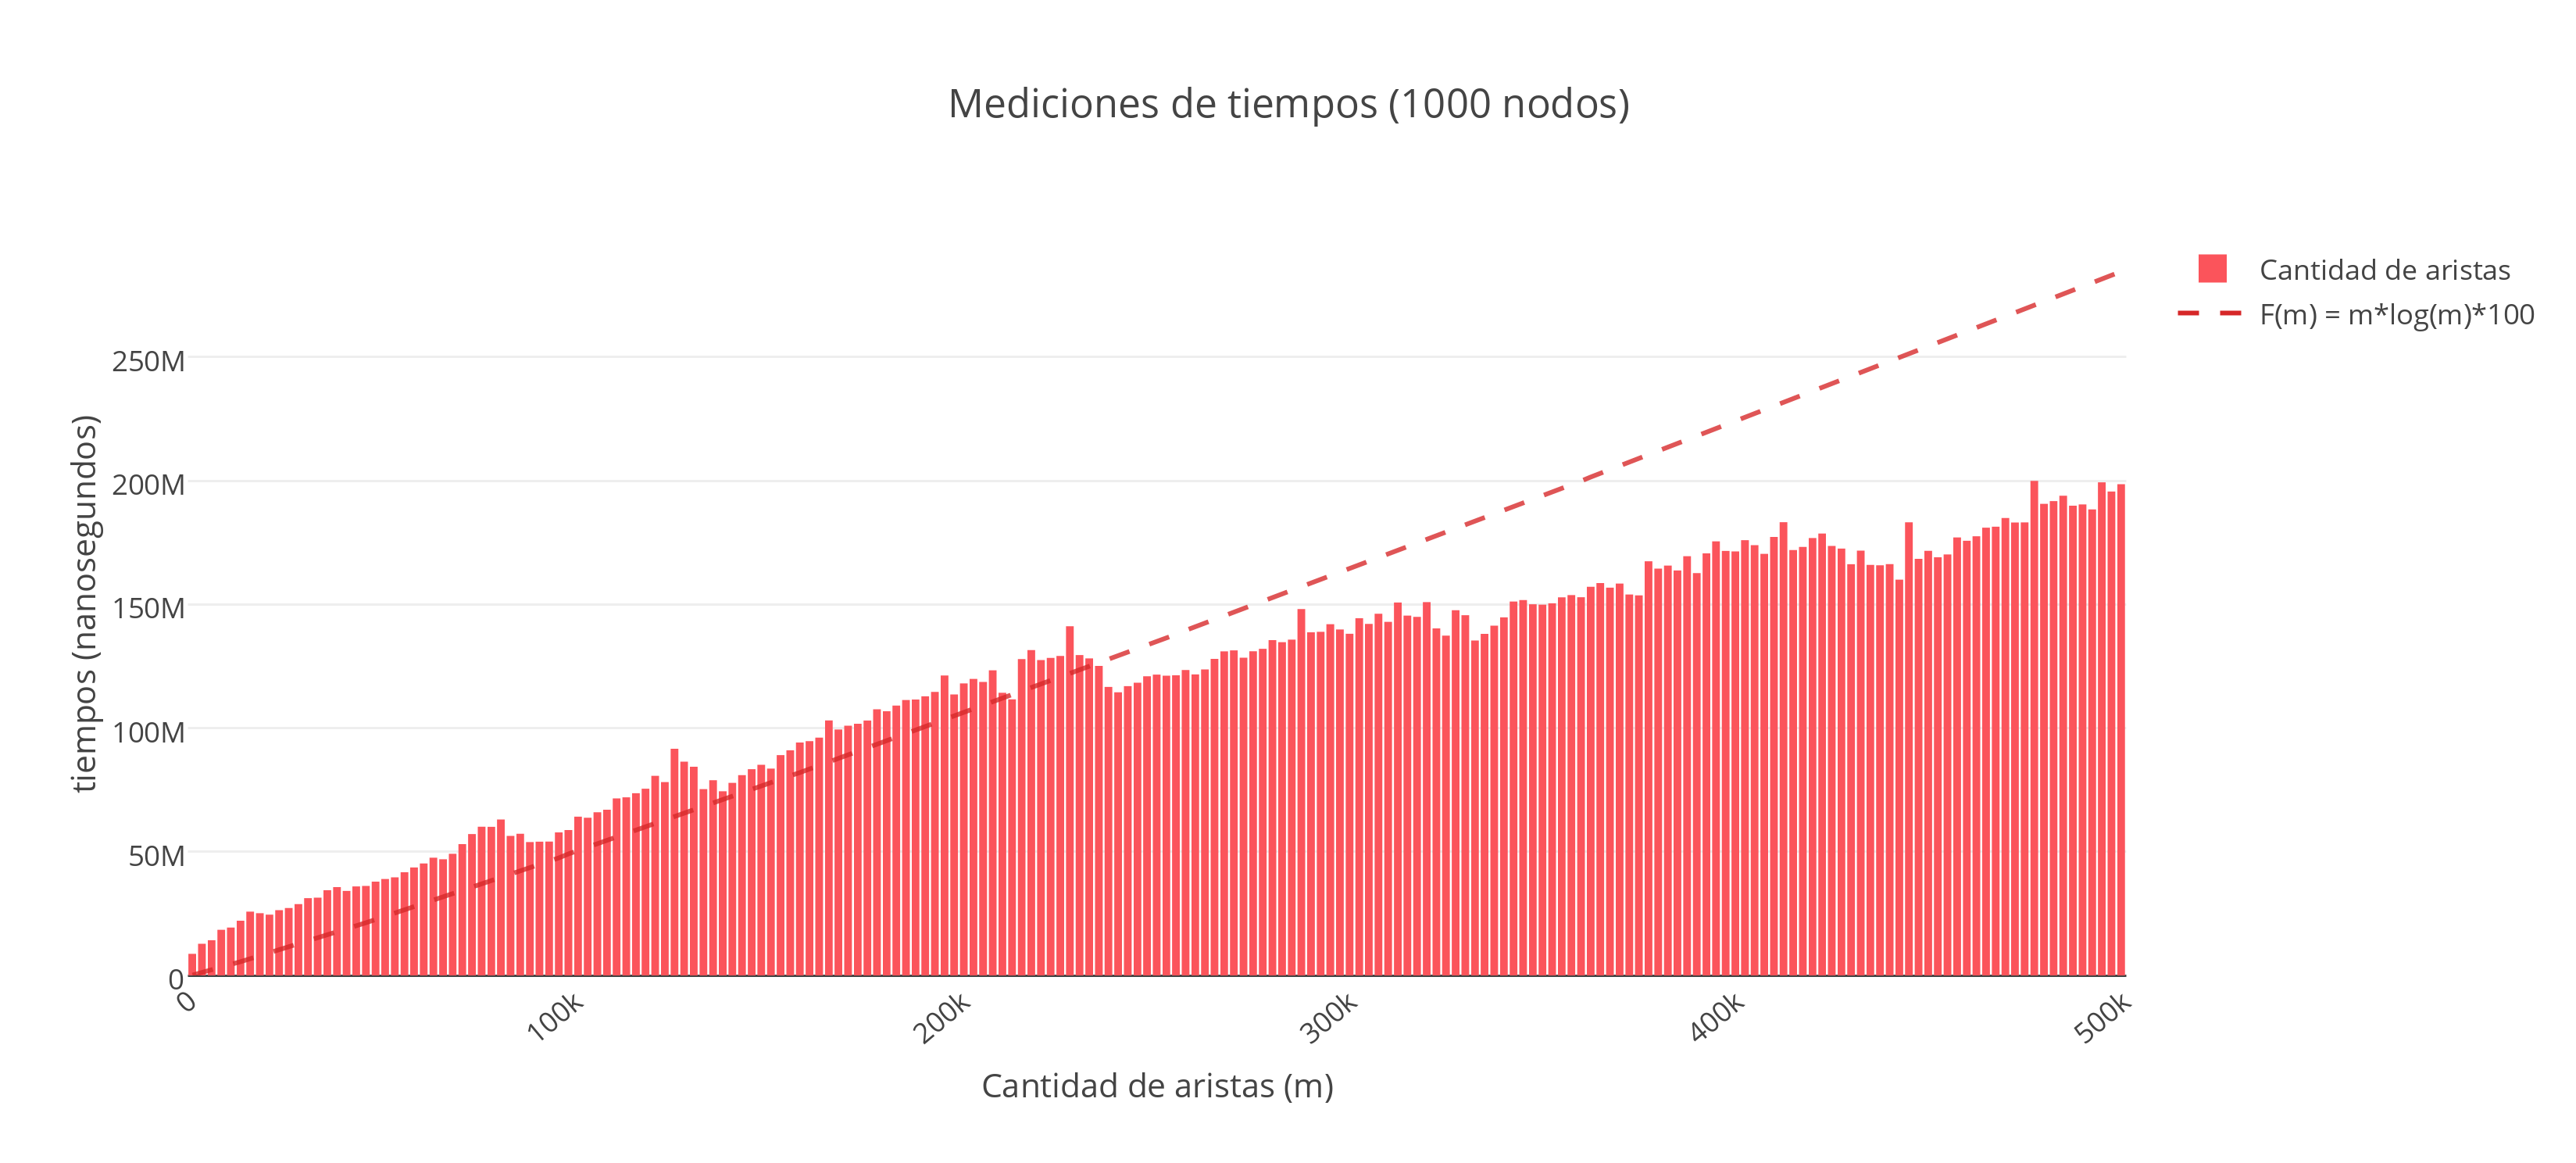
\includegraphics[scale=0.6]{imagenes/ej3/tiempos1000B.png}
% 	\caption{Medición de tiempo promedio con $n$ fijo en 1000}
% 	%\label{tiemposprom}
%  \end{figure}